% !TEX TS-program = pdflatex
% !TEX encoding = UTF-8 Unicode

% This is a simple template for a LaTeX document using the "article" class.
% See "book", "report", "letter" for other types of document.

\documentclass[11pt]{article} % use larger type; default would be 10pt

\usepackage[utf8]{inputenc} % set input encoding (not needed with XeLaTeX)

%%% Examples of Article customizations
% These packages are optional, depending whether you want the features they provide.
% See the LaTeX Companion or other references for full information.

%%% PAGE DIMENSIONS
\usepackage{geometry} % to change the page dimensions
\geometry{a4paper} % or letterpaper (US) or a5paper or....
\geometry{margin=0.5in} % for example, change the margins to 2 inches all round
% \geometry{margin=2in} % for example, change the margins to 2 inches all round
% \geometry{landscape} % set up the page for landscape
%   read geometry.pdf for detailed page layout information

\usepackage{graphicx} % support the \includegraphics command and options

% \usepackage[parfill]{parskip} % Activate to begin paragraphs with an empty line rather than an indent

%%% PACKAGES
\usepackage{booktabs} % for much better looking tables
\usepackage{array} % for better arrays (eg matrices) in maths
\usepackage{paralist} % very flexible & customisable lists (eg. enumerate/itemize, etc.)
\usepackage{verbatim} % adds environment for commenting out blocks of text & for better verbatim
\usepackage{subfig} % make it possible to include more than one captioned figure/table in a single float
% These packages are all incorporated in the memoir class to one degree or another...

%%% HEADERS & FOOTERS
\usepackage{fancyhdr} % This should be set AFTER setting up the page geometry
\pagestyle{fancy} % options: empty , plain , fancy
\renewcommand{\headrulewidth}{0pt} % customise the layout...
\lhead{}\chead{}\rhead{}
\lfoot{}\cfoot{\thepage}\rfoot{}

%%% SECTION TITLE APPEARANCE
\usepackage{sectsty}
\allsectionsfont{\sffamily\mdseries\upshape} % (See the fntguide.pdf for font help)
% (This matches ConTeXt defaults)

%%% ToC (table of contents) APPEARANCE
\usepackage[nottoc,notlof,notlot]{tocbibind} % Put the bibliography in the ToC
\usepackage[titles,subfigure]{tocloft} % Alter the style of the Table of Contents
\renewcommand{\cftsecfont}{\rmfamily\mdseries\upshape}
\renewcommand{\cftsecpagefont}{\rmfamily\mdseries\upshape} % No bold!

%%% END Article customizations

%%% The "real" document content comes below...

\title{Week 4 Assignment}
\author{Efeosa Eguavoen - 17324649}
%\date{} % Activate to display a given date or no date (if empty),
         % otherwise the current date is printed 

\begin{document}
\maketitle

\section{(i)}
\subsection{A}
\begin{center}
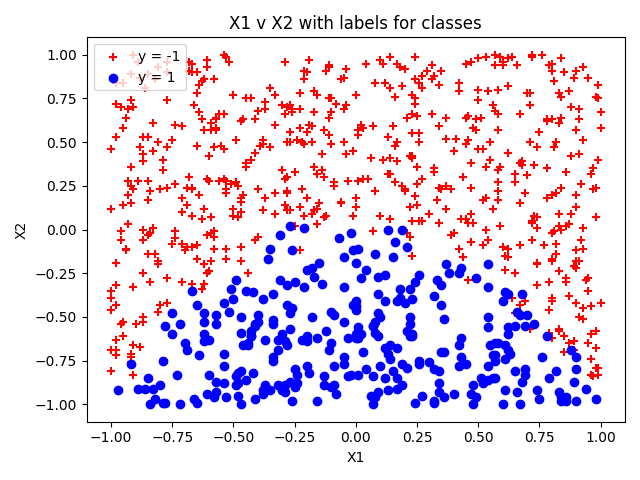
\includegraphics[scale=0.5]{x1vx2.png}
\end{center}
From the above plot, the data is not linealy seperable so some feature engineering will be required to get the correct decision boundary. The decision boundary I would plot based off the above plot would be some sort of quadratic line. 
\begin{center}
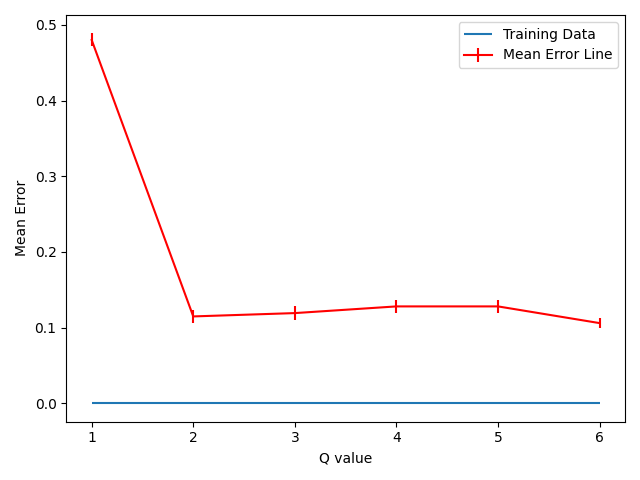
\includegraphics[scale=0.5]{qvalerr.png}
\end{center}
\begin{figure}[h]
\centering
\subfloat[Q =1]{{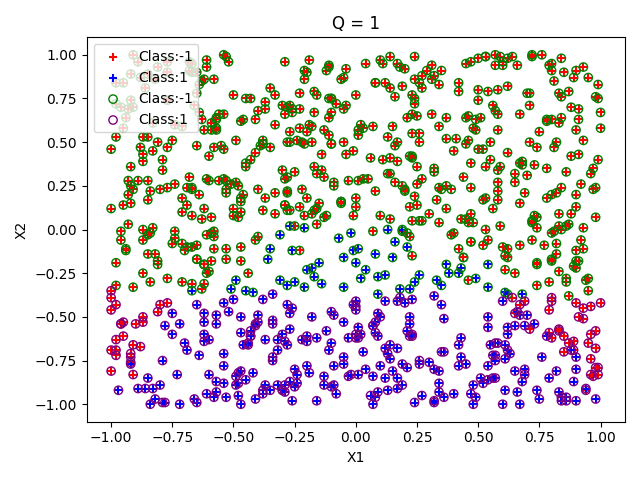
\includegraphics[width=8cm]{s1.png}}}
\qquad
\subfloat[Q = 2]{{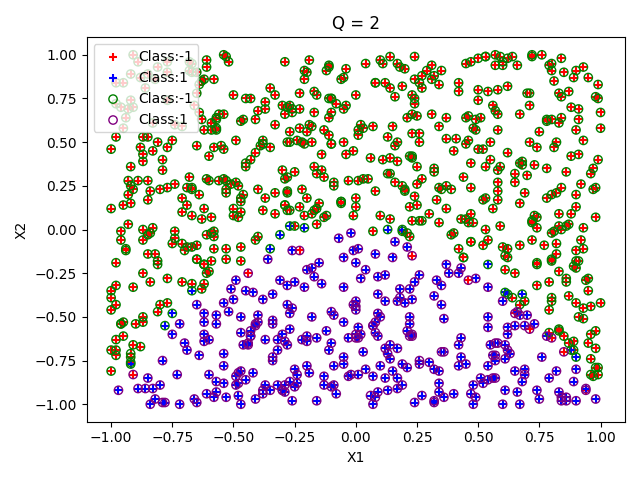
\includegraphics[width=8cm]{s2.png}}}
\qquad
\subfloat[Q = 6]{{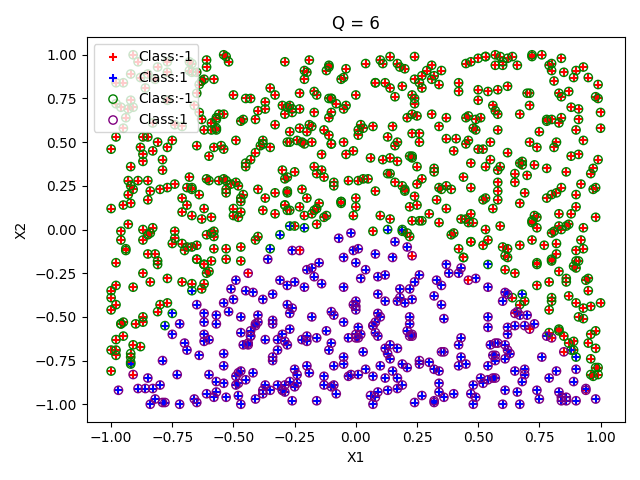
\includegraphics[width=8cm]{s3.png}}}
\qquad
\end{figure}
To select the correct order polynomial to use for my model, I started by looking at my graph to get an estiamate of the order of polynomial that would be required to get the best decision boundary. From the first graph, I knew that it would at least need to be quadratic to I scanned a range of values between 1 and 6 as having too high an order of polynomials would lead to having too many features that would be unnecessary. From the above graph, we can see that when Q = 2 and when Q =6 the mean error is lowest. I went with Q=2 as it's better to keep the model as simple as possible. Above I've also plotted the prediction vs training for different Q values. We can clearly see when Q =1 the data on the bottom right and bottom left corner of the graph has been misclassified. In comparison, when Q =2 and when Q=6 we've gotten much better predictions and much less data has been misclassified. The difference between Q=2 and Q=6 is very little based off the graphs.  \newpage
\begin{figure}[h]
\centering
\subfloat[]{{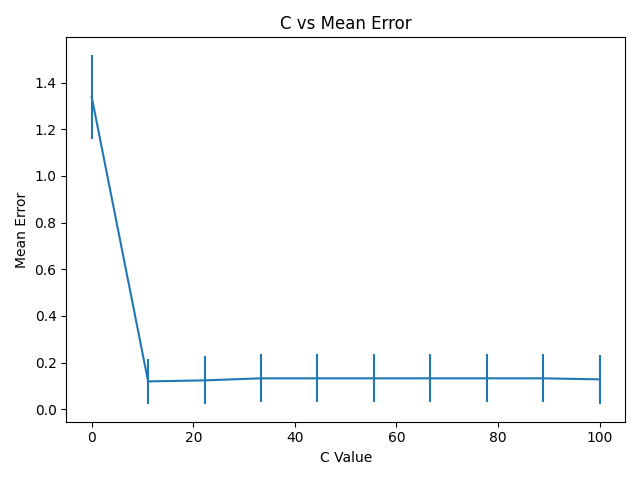
\includegraphics[width=8cm]{c1.png}}}
\qquad
\subfloat[]{{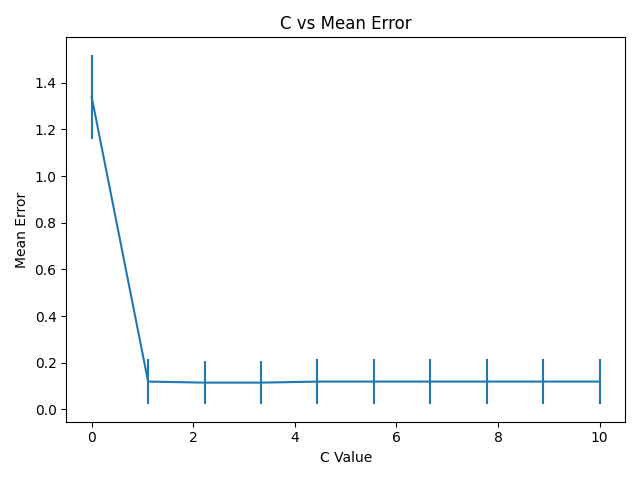
\includegraphics[width=8cm]{c2.png}}}
\qquad
\subfloat[]{{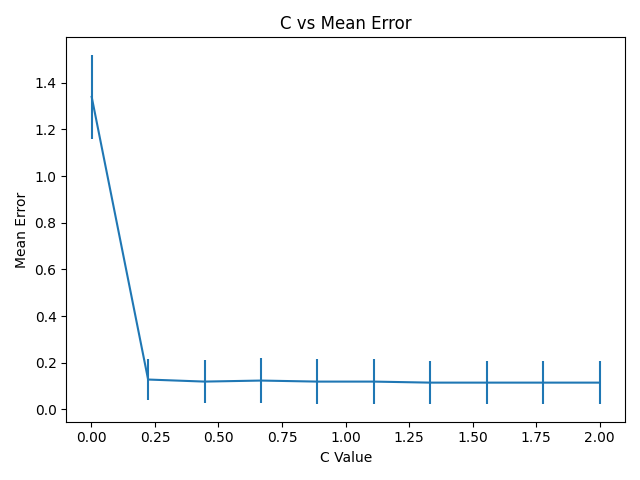
\includegraphics[width=8cm]{c3.png}}}
\qquad
\subfloat[]{{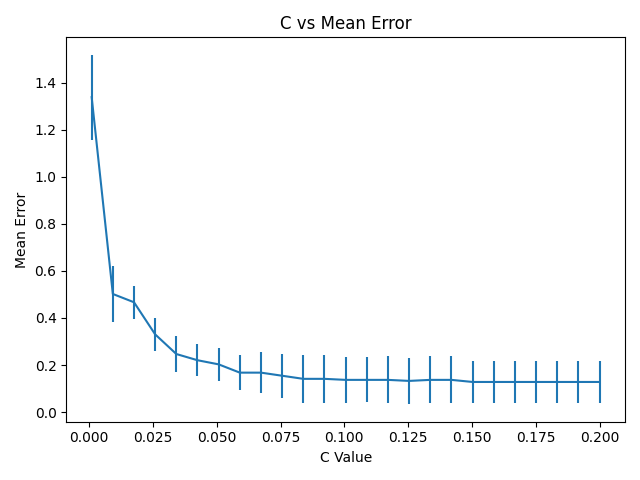
\includegraphics[width=8cm]{c4.png}}}
\end{figure}
To select the correct value of C, I used a range of values of C between 0 and 100 initially to get wide enough spread to select the optimal value of C. From there I reduced the range of values further and further to get the best value of C versus the mean error. From the above graph, C = 0.15 is the optimal value to use for the model as it reduces the error down the most. Higher values of C seem to keep the error around roughly the same value so I just went with the smaller value for simplicity. 
\subsection{B}
\begin{figure}[h]
\centering
\subfloat[K- Large Range]{{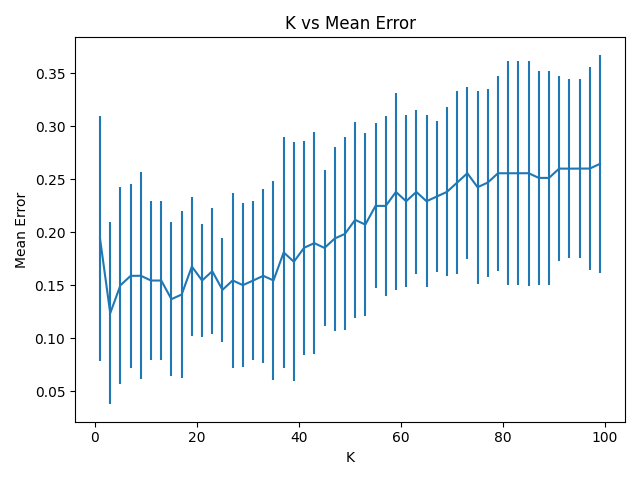
\includegraphics[width=8cm]{k1.png}}}
\qquad
\subfloat[K - Small Range]{{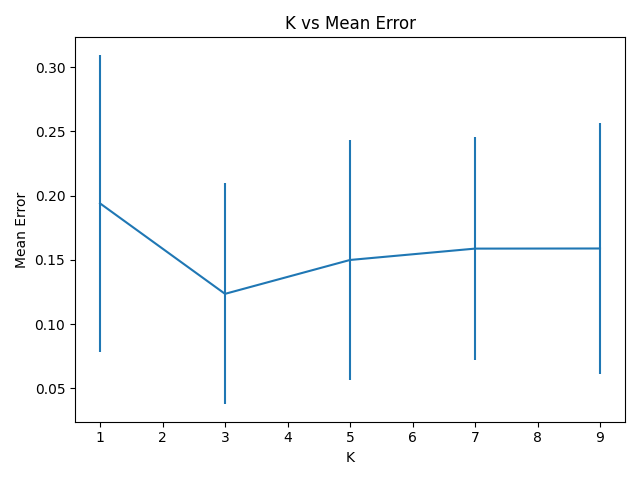
\includegraphics[width=8cm]{k2.png}}}
\qquad
\end{figure}
To select a value for K, I first did some research online about guidelines for calculating K. From what I read, I saw k=sqrt(n). I used this as a baseline for the range of values to search over, so I searched between 1 and 100 initially and from there reduced the range down further. I used cross validation for each value of K, with a k value of k=10. Based on the graphs, above, K = 3 is the optimum value of K to use for the given dataset. The mean error when K = 3 is lowest other than when K = 15 which also has a low error rate. Choosing K = 3 is best as it keeps the model simpler.
\end{document}
